\documentclass[conference]{IEEEtran}
\IEEEoverridecommandlockouts
\usepackage{cite}
\usepackage{amsmath,amssymb,amsfonts}
\usepackage{algorithmic}
\usepackage{graphicx}
\usepackage{textcomp}
\usepackage{xcolor}
\usepackage{url}
\usepackage{array}
\usepackage[hidelinks]{hyperref}
\usepackage{orcidlink}
\newcommand{\mut}{\texorpdfstring{$\mu$}{\textmu}}

\def\BibTeX{{\rm B\kern-.05em{\sc i\kern-.025em b}\kern-.08em
    T\kern-.1667em\lower.7ex\hbox{E}\kern-.125emX}}

\begin{document}

\title{Continual \mut-Training on Edge Devices:\\
A Survey of On-Device Personalisation\thanks{LaTeX
source and the Raspberry~Pi~5 pilot-measurement script
referenced in Section~\ref{sec:challenges} are available at
\url{https://github.com/mklemmingen/ContinualEdgeDevicePersonalisation}.}}

\author{
\IEEEauthorblockN{Marty Lauterbach}
\IEEEauthorblockA{
Reutlingen University\\
Reutlingen, Germany\\
\orcidlink{0009-0007-3396-872X}\,0009-0007-3396-872X
}
}

\maketitle

%---------------------------------------------------------------
\begin{abstract}
Wearable health devices and IoT sensors collect physiological data
that varies between individuals and drifts over time. Pre-trained
models optimised for population-level distributions miss this
variability, while sending raw data or training gradients to the
cloud raises documented privacy risks including Deep Leakage from
Gradients (DLG) attacks. This paper surveys continual on-device
$\mu$-training, in which a small subset of a neural network's
parameters is updated directly on resource-constrained edge
hardware. Recent work on $\mu$-trainers, metaplastic binary
networks, and label-free drift detection is organised along the
four evaluation axes of Huang et al.~\cite{b1}: calculation
complexity, privacy, accuracy, and runtime/energy. The survey
identifies that direct per-update energy measurement on wearable
hardware is missing from every surveyed $\mu$-training source, and
proposes three concrete benchmark targets: per-update energy in
$\mu$J, backward-transfer accuracy on a fixed shift sequence, and
drift-detection latency in samples. A first reproducible reference
data point on Raspberry~Pi-class hardware is reported alongside,
yielding a measured $4.0{\times}$ marginal-energy advantage of
$\mu$-training over full-network training on the same device.
\end{abstract}

\begin{IEEEkeywords}
Wearables, $\mu$-Training, On-Device Learning, Edge AI, Drift
Detection, TinyML, Catastrophic Forgetting
\end{IEEEkeywords}

%---------------------------------------------------------------
\section{Introduction}
\label{sec:intro}

Wearable health devices and IoT sensors generate data shaped by
individual physiological baselines, environmental exposure, and
behavioural patterns. These distributions are also non-stationary:
they drift as sensor hardware ages, user habits evolve, and
biological conditions change. Pre-trained models, regardless of
parameter count, miss this individual-level variability when
deployed in personalised contexts; a model trained on
population-level electrocardiogram (ECG) data degrades on a
specific user's morphology, especially for rare events. Continuous
personalisation at deployment is therefore necessary.

Sending physiological data to the cloud raises privacy concerns.
Even when only weight updates are transmitted, as in standard
federated learning~\cite{FedAvg}, those updates remain vulnerable
to Deep Leakage from Gradients (DLG) attacks~\cite{b8} and
subsequent gradient-inversion variants~\cite{Geiping}, in which
an adversary reconstructs training samples from intercepted
update matrices. On-device adaptation localises the entire learning
process within the device boundary and eliminates this attack
surface, but it must operate inside microcontroller memory and
energy budgets measured in kilobytes of static RAM and microjoules
per operation. Foundational TinyML work has progressively
moved from CNN inference on commodity microcontrollers~\cite{MCUNet},
through activation-memory-aware on-device transfer~\cite{TinyTL},
to full backpropagation training within tight SRAM
budgets~\cite{TinyTrainEng}; the $\mu$-training line surveyed
here continues this trajectory for personalisation rather than
from-scratch training.

\subsection{Contribution}

This paper makes two contributions. First, it synthesises recent
work on on-device $\mu$-trainers, metaplastic binary networks,
and label-free drift detection along the four evaluation axes of
Huang et al.~\cite{b1}; we extend their three-axis framing
(accuracy, energy, resource) by elevating privacy to a fourth
axis and adding non-medical methods (UDDA-TC~\cite{b6}, metaplastic
BNNs~\cite{b9}). Second, it proposes three benchmark targets for cross-study comparison
of on-device $\mu$-training methods: (i) per-update energy in
$\mu$J on a named ARM Cortex-class platform, (ii) catastrophic-forgetting
resistance measured as backward-transfer accuracy (BWT, the
average change in accuracy on previously seen tasks after a new
on-device update; negative values indicate forgetting)
on a fixed sequence of distribution shifts, and (iii)
drift-detection latency in samples between shift onset and the
detector's first positive. Federated personalisation~\cite{b4} is
a complementary direction not surveyed here in detail. The
$\mu$-training literature is currently dominated by a single
research group~\cite{b1,b3,b13}; independent reproductions remain
open.

%---------------------------------------------------------------
\section{Evaluation Framework}
\label{sec:framework}

We adopt a four-axis extension of the framing in~\cite{b1}:
\textbf{calculation complexity}, \textbf{privacy}, \textbf{accuracy
and generalisation}, and \textbf{runtime/energy}. Privacy is
elevated to a first-class axis because gradient-egress
vulnerability~\cite{b8} is a core motivation for on-device
adaptation; runtime and energy are kept on a single axis because
every primary source's energy figure is reported on a specific
hardware platform and is therefore inseparable from runtime.

\textbf{Calculation complexity} covers memory for weights,
intermediate layer activations, and the gradients computed during
training. Standard architectures need hundreds of megabytes for one
forward pass, ruling out on-device training on commodity
microcontrollers without aggressive quantisation (storing each
weight in fewer bits than the standard 32-bit float to shrink
memory and compute); a 6-bit quantised compact CNN deployed on
dedicated low-power hardware~\cite{b10} achieves 0.350\,$\mu$J per
inference at 0.140\,ms latency.

\textbf{Privacy} captures whether raw data, intermediate
activations, or training updates leave the device. Updates alone
remain vulnerable to gradient-inversion~\cite{b8,Geiping}.

\textbf{Runtime and energy} together determine deployability.
Training a model on-device costs orders of magnitude more energy
than running it for inference, so on-device adaptation must be
event-driven rather than continuous.

\textbf{Accuracy and generalisation} justify any adaptation cycle:
an update is worth its energy cost only when it produces a
measurable accuracy gain on the user's distribution. Optimising
one axis tends to compromise others.

%---------------------------------------------------------------
\section{On-Device \mut-Trainers}
\label{sec:mutrainers}

The most conservative on-device adaptation strategy freezes every
layer of the pre-trained network except the final classifier and
updates only that layer, restricting computation to the final
feature vector and class logits. This last-layer calibration works
for transfer scenarios where the deployment distribution is
semantically aligned with the pre-training distribution, but its
limitation is that frozen feature-extraction layers cannot acquire
genuinely new representations. BioTrain~\cite{BioTrain}
measures the gap directly: on EEG and EOG new-subject calibration,
full-network fine-tuning outperforms last-layer updates by
approximately 7~percentage points of accuracy on a low-power
microcontroller under a sub-50\,mW power budget.

The main line of work in on-device personalisation extends
this idea by selecting a small subset of \emph{intermediate}
layers as trainable while keeping the rest \emph{frozen} (frozen
layers receive no weight updates and contribute no gradients,
so neither their values nor the intermediate activations needed
to compute their gradients have to be stored on-device). Developed
by Huang et al.~\cite{b3,b13} for secure real-time processing of
medical signals (continuous ECG and electroencephalogram
monitoring), this $\mu$-training approach recovers more
representational flexibility than last-layer calibration without
paying the full memory cost of training every layer.

\subsection{Tripartite Pipeline}

The original $\mu$-trainer follows a three-phase pipeline.

\textit{Phase~1: Full Cloud Training.} A compact model is trained
on a large aggregated dataset, e.g. the Telehealth Network of
Minas Gerais ECG repository~\cite{b3}. The model is structured in
three blocks: an input encoder, an intermediate processing layer,
and an output decoder.

\textit{Phase~2: $\mu$-Training (pre-deployment).} Encoder and
decoder are initialised from the trained foundational model and
frozen; only the middle layer is updated. The original middle-layer
training used a separate, larger teacher network as a supervision
target~\cite{b3}; the follow-up work~\cite{b13} eliminates the
on-device teacher by using the model as its own teacher
(\emph{self-distillation}).

\textit{Phase~3: On-Device $\mu$-Fine-Tuning.} Once deployed
(evaluated on Raspberry~Pi~3 Model~B~\cite{b3} and
Radxa~Zero~\cite{b13}), the freezing logic inverts: the middle
layer is frozen to preserve its distilled representations while
the encoder and decoder are unfrozen and updated on personal data
when user-specific drift is detected.

\subsection{Parameter Efficiency and Privacy}

$\mu$-trainers work because the on-device trainable subset is
small. For the specific 6.4\,M-parameter CNN
foundational model evaluated in~\cite{b3}, less than 2\,\% of
weights are updated on-device; the absolute fraction is
architecture-dependent but the order of magnitude is
representative. Updates fit within on-chip memory, avoiding
off-chip data transfers and remaining within microjoule energy
budgets.

Localising raw data, activations, and weight updates within the
device boundary eliminates the attack surface for gradient-inversion
attacks~\cite{b8}. Because the device does not send updates to a
global aggregator, the entire DLG attack family is inapplicable
by construction, giving a strong privacy guarantee for regulated
health data.

%---------------------------------------------------------------
\section{Catastrophic Forgetting and Metaplastic BNNs}
\label{sec:forgetting}

Continual on-device updates risk overwriting safety-critical
features: an ECG monitor that adapts its weights to a user's
resting heart-rate variability could overwrite the parameters
needed to detect rare arrhythmic events. Standard mitigations
(replay buffers that rehearse stored past samples alongside new
data~\cite{iCaRL}, and importance-weighted regularisation that
protects weights deemed important to past tasks~\cite{EWC}) both
add memory or compute that wearable microcontrollers cannot spare.

Drawing on neuroscience, Laborieux et al.~\cite{b9} propose Binary
Neural Networks (BNNs) as a forgetting-resistant on-device
substrate. BNNs constrain weights to $\pm 1$ at inference time,
allowing integer-only operations rather than floating-point
arithmetic; training nonetheless accumulates small updates in a
hidden real-valued shadow per binary weight, binarised only at the
inference boundary. Laborieux et al.\ reinterpret that shadow's
magnitude as a per-weight stability score: weights with large
hidden magnitudes become progressively resistant to flipping while
small-magnitude weights remain plastic. The same architectural
mechanism that gives efficient inference also gives forgetting
resistance, without the memory overhead of replay or the compute
overhead of~\cite{EWC}. The result is demonstrated on multitask
and stream-learning vision benchmarks; demonstration on streaming
physiological signals (ECG, EEG, IMU) remains an open empirical
step.

%---------------------------------------------------------------
\section{Label-Free Drift Detection}
\label{sec:drift}

On-device adaptation cannot run continuously without exhausting
the energy budget; updates must be triggered by statistically
significant changes in the data distribution. In deployed edge
systems, distributions drift continuously as user behaviour and
sensor characteristics change.
Classical streaming drift detectors (DDM~\cite{DDM},
CUSUM-based change-point methods) mostly
assume access to ground-truth labels for incoming data, which is
impractical on a wearable where the user cannot annotate their own
physiological stream in real time. Label-free drift detection is
therefore a precondition for autonomous on-device adaptation.

The Unsupervised Real-Time Drift Detection and Adaptation method
for continual Traffic Classification (UDDA-TC)~\cite{b6} implements a
two-tier detector. The first tier is a sliding-window adaptive
weighted CUSUM detector: it accumulates small deviations from an
expected mean and signals when the cumulative breach exceeds a
threshold, indicating sustained shift rather than noise, with the
sliding window bounding memory consumption. The second tier introduces a Weighted Logits Variation (WLV)
signal. Logits are the model's raw per-class prediction scores
before softmax normalisation; WLV aggregates the variance of these
scores over a sliding window, weighted by class prior. The
resulting one-dimensional signal serves as a proxy for input
drift, computable on edge hardware where direct distributional
analysis of high-dimensional inputs would be prohibitive. On joint detection, the system
reconstructs a training set by merging the emerging distribution
with retained anchor points from the historical distribution,
producing a compact batch suitable for a subsequent
$\mu$-fine-tuning cycle.

A complementary line of work places the detection target inside
the network rather than on its inputs or outputs. Three published
frameworks instantiate this idea along distinct signals:
prototype-distance in a contrastive latent space~\cite{CADE},
distribution distance over a sliding representation
window~\cite{DriftLens}, and trajectory deviation in the DIKWP
semantic-transformation framework of Mei et al.~\cite{b7}. These
detectors could complement UDDA-TC's output-side trigger by
catching shifts that affect intermediate representations before
they reach the prediction layer, but none has been validated on
wearable microcontroller hardware; for that reason they are not
included as separate rows in the comparative analysis of
Section~\ref{sec:comparison}, and their adaptation to the
$\mu$-training setting has not yet been attempted.

%---------------------------------------------------------------
\section{Comparative Analysis}
\label{sec:comparison}

Table~\ref{tab:comparison} summarises the surveyed methods across
the four axes of Section~\ref{sec:framework}. Cross-row magnitudes
compare design properties rather than benchmark performance (rows
span biosignals, vision, and encrypted traffic); cells where the
source does not report a comparable metric are qualitative.

\begin{table*}[t]
\caption{Comparative Analysis of On-Device Adaptation Methodologies}
\label{tab:comparison}
\centering
\renewcommand{\arraystretch}{1.05}
\small
\begin{tabular}{|>{\bfseries}p{2.4cm}|p{2.9cm}|p{2.5cm}|p{3.5cm}|p{3.5cm}|}
\hline
\textbf{Approach} &
\textbf{Calculation Complexity} &
\textbf{Privacy} &
\textbf{Accuracy \& Generalisation} &
\textbf{Runtime \& Energy} \\
\hline
$\mu$-Training~\cite{b3,b13} &
Very Low ($<$2\,\% of weights updated, architecture-dependent~\cite{b3}) &
Very High (no update egress) &
Improved over static foundational model on TNMG/CPSC ECG~\cite{b3} &
On-chip updates on Raspberry~Pi~3~\cite{b3} and Radxa~Zero~\cite{b13}; this work measures 33.8\,ms/118\,mJ per update on Pi~5 (4.0$\times$ less than full-network) \\
\hline
Metaplastic BNN~\cite{b9} &
Ultra-Low (integer-only operations) &
High (binary weights obfuscate raw input) &
Matches~\cite{EWC} on permuted-MNIST and similar multitask benchmarks~\cite{b9}; no physiological evaluation reported &
Efficient inference; per-update $\mu$J figure not reported \\
\hline
Label-Free Drift (UDDA-TC)~\cite{b6} &
Low (logit variance + sliding window) &
High (fully unsupervised; no label egress) &
Drift-detection F1 0.71--0.76 across three traffic-classification corpora~\cite{b6} &
Sliding-window bounds memory; per-decision compute comparable to baseline change detectors \\
\hline
\end{tabular}
\end{table*}

When privacy and calculation complexity dominate, as in implanted
medical devices or secure hearable biosensors, $\mu$-training is
the current state of the art: less than 2\,\% of model parameters
are updated, operations fit within on-chip memory, and update
egress is eliminated~\cite{b3,b13}. For workloads needing continuous real-time runtime alongside
forgetting resistance, metaplastic BNNs are the architectural
candidate, though their
empirical case has been made on vision streams rather than on
physiological time series~\cite{b9}. Label-free drift detection is a necessary auxiliary regardless of
the core adaptation algorithm: adaptation is energetically viable
only when triggered by genuine distributional shift~\cite{b6}.

%---------------------------------------------------------------
\section{Open Challenges and Quantitative Bounds}
\label{sec:challenges}

\begin{figure}[t]
\centering
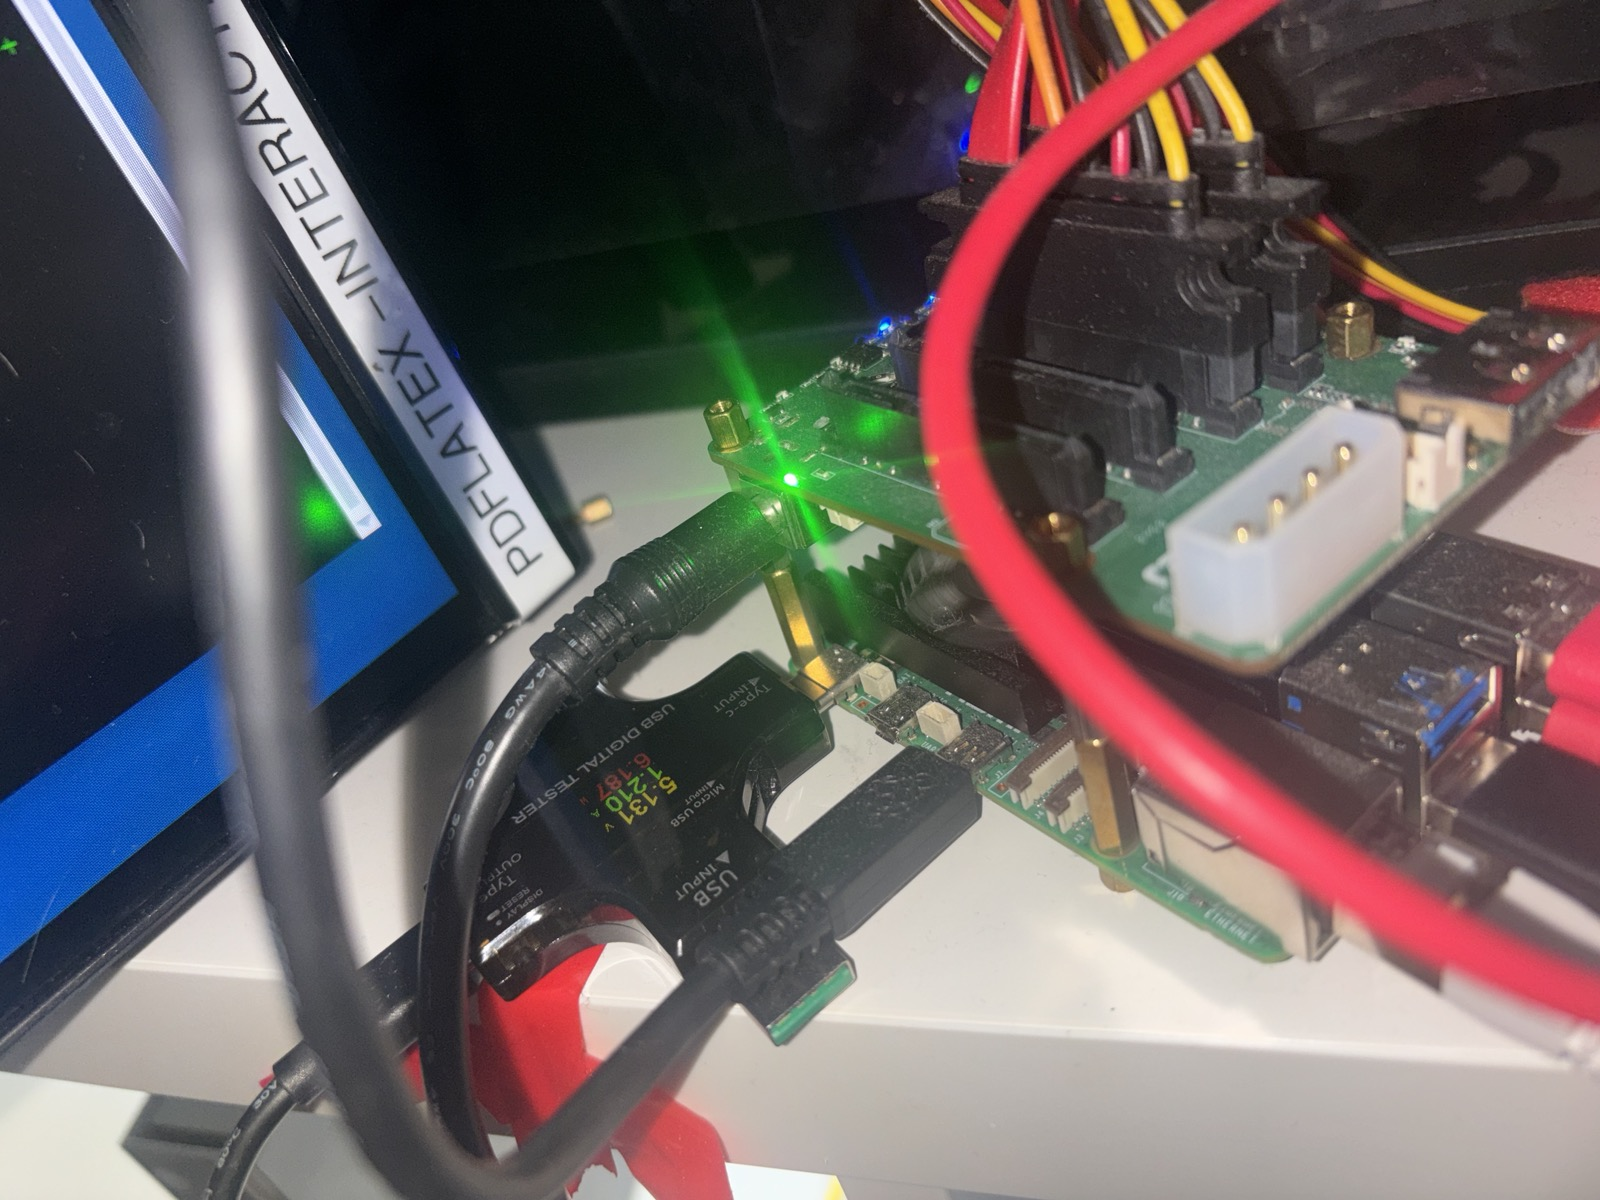
\includegraphics[width=0.78\columnwidth]{pilot/IMG_3825.jpg}
\caption{Pilot-measurement testbed referenced by the data point in
the energy-asymmetry discussion below. A Raspberry~Pi~5 hosts the
$\mu$-training, inference, and drift-detection workloads. The
ATORCH J7-c USB-C inline meter visible in the foreground (reading
5.13\,V, 1.07\,A) is used as a sanity-check reference; the reported
power figures themselves come from the Pi~5's on-chip Renesas
DA9091 PMIC, queried via \texttt{vcgencmd pmic\_read\_adc}. The
PMIC measures the secondary rails it generates (3V3, 1V8,
VDD\_CORE, DDR, $\ldots$) but not the 5\,V main-rail current
directly, so peripheral draw (HAT, fan, and cabling visible in
frame) is excluded from totals; relative comparisons across phases
remain valid because the unmeasured offset is approximately
constant.}
\label{fig:testbed}
\end{figure}

\textit{Catastrophic forgetting under tight memory.} Partial
freezing and metaplasticity offer pathways but have not been
validated end-to-end on streaming physiological signals over long
horizons. Cross-modality demonstration on ECG, EEG, or IMU streams
remains the open empirical step for both $\mu$-trainers and
metaplastic BNNs~\cite{b9}. As a sanity check on the methodology
proposed below in (ii), we ran a synthetic two-task forgetting
probe on the same Pi~5 testbed, scored with the backward-transfer
(BWT) metric of Lopez-Paz \& Ranzato~\cite{GEM} (input mean shift
and label rotation between tasks for the synthetic construction):
full-network training collapses to BWT$=-1.0$ (complete forgetting
of task~0 after training on task~1), confirming that the failure
mode targeted by $\mu$-training and metaplasticity is real and
immediately reproducible on commodity hardware.

\textit{Energy asymmetry between inference and training.}
Inference is efficient: 0.350\,$\mu$J at 0.140\,ms latency on
dedicated low-power hardware~\cite{b10}, well within the energy
budget of a wearable-class battery for continuous monitoring.
The corresponding per-update training energy is not directly
reported in any of the surveyed $\mu$-training sources. The wider
TinyML training literature provides reference points that bracket
the achievable measurement envelope: per-iteration training energy
on low-end~\cite{POET} and mid-range~\cite{PockEngine}
microcontrollers, and full-network biosignal fine-tuning under
50\,mW on the GAP9 RISC-V MCU~\cite{BioTrain}.

To anchor this gap with a first reproducible reference point on the
same Pi-class hardware that the surveyed $\mu$-training works
deploy on (Raspberry~Pi~3~\cite{b3}, Radxa~Zero~\cite{b13}), we
ran the testbed of Fig.~\ref{fig:testbed} through a
trainable-fraction sweep on a Raspberry~Pi~5 with on-chip PMIC
power telemetry (via \texttt{vcgencmd pmic\_read\_adc}). With the
$\mu$-training freeze pattern (2.06\,\% of weights trainable on a
99.7\,k-parameter ECG-shaped 1D-CNN), each update costs 33.8\,ms
and 118\,mJ above the 2.77\,W Pi~5 idle baseline, versus 137.9\,ms
and 475\,mJ for full-network training: a $4.08{\times}$ wall-time
and $4.02{\times}$ marginal-energy advantage measured on the same
device (Fig.~\ref{fig:sweep}). The Pi~5 measurement sits 3--4
orders of magnitude above the $10^{2}\,\mu$J/update Cortex-M
target proposed below; the next step is to repeat the sweep on
Cortex-M4F/M7 hardware to close the gap.

\begin{figure}[!htbp]
\centering
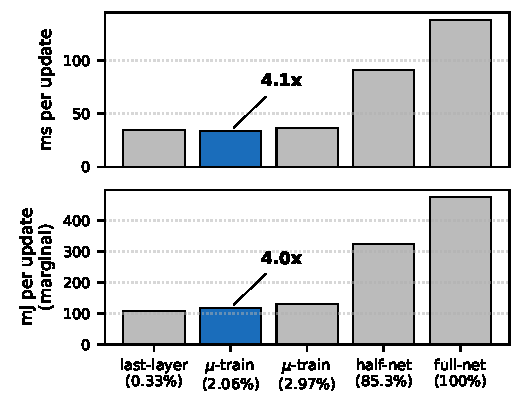
\includegraphics[width=\columnwidth]{pilot/fig_trainable_sweep.pdf}
\caption{Per-update wall-time (top) and marginal energy above the
2.77\,W Pi~5 idle baseline (bottom) versus trainable-parameter
fraction. The $\mu$-training operating point at 2.06\,\% trainable
(blue) sits on the flat regime; the cost climbs sharply above
${\sim}3\,\%$ trainable as additional convolutional layers enter
the backward pass. Annotations give the measured $\mu$-training
vs.\ full-network ratios. Raspberry~Pi~5, 4 threads, batch~32,
seq.~length~250, FP32, SGD; PMIC-summed power excludes
peripherals on the unmeasured 5\,V main rail (see
Fig.~\ref{fig:testbed} caveat).}
\label{fig:sweep}
\end{figure}

\begin{figure*}[t]
\centering
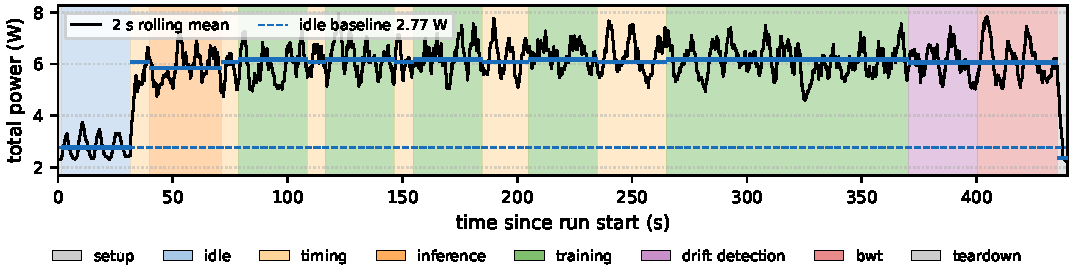
\includegraphics[width=\textwidth]{pilot/fig_power_timeline.pdf}
\caption{Power telemetry over the full 440\,s pilot run. Background
colour bands indicate the active pipeline phase (legend below);
the thin grey trace is raw 5\,Hz PMIC samples
(\texttt{vcgencmd pmic\_read\_adc} summed across the 14 measured
rails) and the thick black trace is a 2\,s rolling mean. Short
blue horizontal segments are per-phase mean-power overlays; the
dashed line is the 2.77\,W idle reference. The trainable-fraction
sweep is visible as the five training plateaus near the centre,
with the largest two (\textit{half-net} and \textit{full-net})
distinguishable by their longer settle time per update.}
\label{fig:timeline}
\end{figure*}

\textit{Label-free drift-detection calibration.} The two-tier
UDDA-TC detector bounds memory and compute, but its threshold
parameters are tuned empirically rather than derived. UDDA-TC
reports drift-detection F1 in the range 0.71--0.76 on three
traffic-classification corpora~\cite{b6}, leaving open the question
of robustness on high-noise wearable signals where distributional
shift is gradual rather than abrupt. Our Pi~5 implementation of
a UDDA-TC-style WLV+CUSUM detector adds 36.6\,ms and 121\,mJ per
decision (above idle), within $3\,\%$ of the cost of a plain FP32
inference call on the same network: detector overhead is
negligible at this scale, so the cost driver remains the
inference itself, not the drift signal.

\textit{Toward a shared benchmark.} Three concrete targets:
(i)~per-update energy in $\mu$J on a named ARM Cortex-class
platform (e.g.\ Cortex-M4F or Cortex-M7). One ``update'' is the
parameter-update sequence triggered by a single detected drift
event: typically one mini-batch over the new-data window plus
retained anchor points. Optimizer state, the auxiliary memory used
by the training algorithm itself such as Adam's per-weight running
averages, is held constant across compared methods. A working
ceiling on the order of $10^{2}\,\mu$J/update is consistent with
the multi-day continuous-operation budget of a 320\,mAh-class
wearable cell~\cite{b10}.
(ii)~Catastrophic forgetting measured as backward-transfer
accuracy on a fixed sequence of $\geq 5$ distribution shifts, for
example a held-out subject sequence from a public biosignal corpus
such as MIT-BIH (ECG) or PhysioNet 2017, with the shift schedule
and anchor-retention policy fixed across methods.
(iii)~Drift-detection latency, measured in samples between a
labelled shift onset and the detector's first positive, reported
at a fixed operating point (the threshold yielding a 0.05
false-positive rate over a no-shift control window of fixed
length, e.g.\ 10{,}000 samples) so that latency cannot be reduced
by accepting more false alarms.

%---------------------------------------------------------------
\section{Conclusion}
\label{sec:conclusion}

Inference at sub-millisecond latency and sub-microjoule
per-inference cost has been demonstrated on dedicated low-power
hardware~\cite{b10}; the corresponding per-update training figures
for the surveyed $\mu$-training methods have not been reported.
The Pi~5 reference point measured in Section~\ref{sec:challenges}
gives a $4.0{\times}$ $\mu$-training-over-full-network advantage on
commodity hardware; the three benchmark targets proposed there are
tractable next measurement steps that would enable direct
cross-study comparison on Cortex-M-class targets.

%---------------------------------------------------------------
\begin{thebibliography}{00}

\bibitem{b1}
Z.~Huang, L.~Yu, L.~F.~H.~Contreras, G.~Dwivedi, and O.~Kavehei,
``On-device machine learning for secure, generalizable and real-time
medical data processing: on the emergence of $\mu$-trainers,''
\textit{Royal Society Open Science}, vol.~12, no.~12, p.~251213,
Dec. 2025.

\bibitem{b3}
Z.~Huang, L.~Yu, L.~F.~H.~Contreras, K.~Eshraghian, N.~D.~Truong,
A.~Nikpour, and O.~Kavehei,
``Advancing privacy-aware machine learning on sensitive data via
edge-based continual $\mu$-training for personalized large models,''
\textit{Machine Learning: Science and Technology}, vol.~6, no.~1,
p.~015025, Jan. 2025,
doi: \href{https://doi.org/10.1088/2632-2153/adaca3}{10.1088/2632-2153/adaca3}.

\bibitem{b4}
H.~Lin, L.~Shou, K.~Chen, G.~Chen, and S.~Wu,
``LINDT: Tackling negative federated learning with local adaptation,''
\textit{arXiv preprint} \href{https://arxiv.org/abs/2011.11160}{arXiv:2011.11160} [cs.LG], Nov. 2020.

\bibitem{b6}
M.~Liu, P.~Wang, Z.~Li, Y.~Ye, Z.~Wang, and X.~Chen,
``UDDA-TC: Unsupervised real-time drift detection and adaptation for
continual traffic classification in mobile edge computing,''
\textit{IEEE Transactions on Consumer Electronics}, early access,
2025, doi: \href{https://doi.org/10.1109/TCE.2025.3579882}{10.1109/TCE.2025.3579882}.

\bibitem{b7}
Y.~Mei, Y.~Duan, K.~Wu, and Y.~Li,
``A DIKWP white-box semantic distributed learning approach for
resource-constrained edge devices in web environments,''
\textit{International Journal of Web Information Systems},
vol.~22, no.~1, pp.~17--43, 2026,
doi: \href{https://doi.org/10.1108/IJWIS-06-2025-0142}{10.1108/IJWIS-06-2025-0142}.

\bibitem{b8}
L.~Zhu, Z.~Liu, and S.~Han,
``Deep leakage from gradients,''
in \textit{Advances in Neural Information Processing Systems
(NeurIPS)}, vol.~32, 2019.

\bibitem{b9}
A.~Laborieux, M.~Ernoult, T.~Hirtzlin, and D.~Querlioz,
``Synaptic metaplasticity in binarized neural networks,''
\textit{Nature Communications}, vol.~12, no.~2549, May 2021,
doi: \href{https://doi.org/10.1038/s41467-021-22768-y}{10.1038/s41467-021-22768-y}.

\bibitem{b10}
T.~Ling, C.~Qian, P.~Zdankin, T.~Weis, and G.~Schiele,
``StrikeWatch: Wrist-worn gait recognition with compact time-series
models on low-power FPGAs,''
in \textit{Proc. 2025 IEEE Annual Congress on Artificial Intelligence
of Things (AIoT)}, Dec. 2025, pp.~66--74,
doi: \href{https://doi.org/10.1109/aiot66900.2025.00021}{10.1109/aiot66900.2025.00021}.

\bibitem{b13}
Z.~Huang, L.~Yu, L.~F.~Herbozo Contreras, and O.~Kavehei,
``Efficient and secure $\mu$-Training and $\mu$-Fine-Tuning for
edge-based TinyML with future-guided self-distillation,''
\textit{Mach. Learn.: Health}, vol.~1, no.~1, p.~015002, Jul. 2025,
doi: \href{https://doi.org/10.1088/3049-477X/add26a}{10.1088/3049-477X/add26a}.

\bibitem{EWC}
J.~Kirkpatrick et al.,
``Overcoming catastrophic forgetting in neural networks,''
\textit{Proc. National Academy of Sciences (PNAS)},
vol.~114, no.~13, pp.~3521--3526, 2017,
doi: \href{https://doi.org/10.1073/pnas.1611835114}{10.1073/pnas.1611835114}.

\bibitem{CADE}
L.~Yang, W.~Guo, Q.~Hao, A.~Ciptadi, A.~Ahmadzadeh, X.~Xing,
and G.~Wang,
``CADE: Detecting and explaining concept drift samples for
security applications,''
in \textit{Proc. 30th USENIX Security Symposium}, 2021,
pp.~2327--2344.

\bibitem{DriftLens}
S.~Greco, B.~Vacchetti, D.~Apiletti, and T.~Cerquitelli,
``Unsupervised concept drift detection from deep learning
representations in real-time,''
\textit{IEEE Transactions on Knowledge and Data Engineering},
2025. \href{https://arxiv.org/abs/2406.17813}{arXiv:2406.17813}.

\bibitem{BioTrain}
R.~Wang, V.~J.~B.~Jung, P.~Wiese, S.~Frey, G.~Spacone,
F.~Conti, A.~Burrello, and L.~Benini,
``BioTrain: Sub-MB, Sub-50\,mW on-device fine-tuning for Edge-AI on
biosignals,''
in \textit{Proc. 2026 Int. Joint Conf. Neural Networks (IJCNN)},
IEEE, 2026, accepted. \href{https://arxiv.org/abs/2604.13359}{arXiv:2604.13359}.

\bibitem{POET}
S.~G.~Patil, P.~Jain, P.~Dunnmon, N.~Carbin, M.~Rana, and
J.~E.~Gonzalez,
``POET: Training neural networks on tiny devices with integrated
rematerialization and paging,''
in \textit{Proc. 39th Int. Conf. Machine Learning (ICML)},
PMLR, vol.~162, 2022, pp.~17573--17583.

\bibitem{PockEngine}
L.~Zhu, L.~Hu, J.~Lin, W.-C.~Wang, W.-M.~Chen, C.~Gan, and
S.~Han,
``PockEngine: Sparse and efficient fine-tuning in a pocket,''
in \textit{Proc. 56th IEEE/ACM Int. Symp. Microarchitecture
(MICRO)}, 2023, pp.~1381--1396,
doi: \href{https://doi.org/10.1145/3613424.3614307}{10.1145/3613424.3614307}.

\bibitem{MCUNet}
J.~Lin, W.-M.~Chen, Y.~Lin, J.~Cohn, C.~Gan, and S.~Han,
``MCUNet: Tiny deep learning on IoT devices,''
in \textit{Advances in Neural Information Processing Systems
(NeurIPS)}, vol.~33, 2020, pp.~11711--11722.

\bibitem{TinyTL}
H.~Cai, C.~Gan, L.~Zhu, and S.~Han,
``TinyTL: Reduce memory, not parameters for efficient on-device
learning,''
in \textit{Advances in Neural Information Processing Systems
(NeurIPS)}, vol.~33, 2020, pp.~11285--11297.

\bibitem{TinyTrainEng}
J.~Lin, L.~Zhu, W.-M.~Chen, W.-C.~Wang, C.~Gan, and S.~Han,
``On-device training under 256\,KB memory,''
in \textit{Advances in Neural Information Processing Systems
(NeurIPS)}, vol.~35, 2022, pp.~22941--22954.

\bibitem{FedAvg}
H.~B.~McMahan, E.~Moore, D.~Ramage, S.~Hampson, and B.~A.~y~Arcas,
``Communication-efficient learning of deep networks from decentralized
data,''
in \textit{Proc. 20th Int. Conf. Artificial Intelligence and
Statistics (AISTATS)}, PMLR, vol.~54, 2017, pp.~1273--1282.

\bibitem{Geiping}
J.~Geiping, H.~Bauermeister, H.~Dr\"oge, and M.~Moeller,
``Inverting gradients --- how easy is it to break privacy in
federated learning?,''
in \textit{Advances in Neural Information Processing Systems
(NeurIPS)}, vol.~33, 2020, pp.~16937--16947.

\bibitem{iCaRL}
S.-A.~Rebuffi, A.~Kolesnikov, G.~Sperl, and C.~H.~Lampert,
``iCaRL: Incremental classifier and representation learning,''
in \textit{Proc. IEEE Conf. Computer Vision and Pattern Recognition
(CVPR)}, 2017, pp.~5533--5542.

\bibitem{DDM}
J.~Gama, P.~Medas, G.~Castillo, and P.~Rodrigues,
``Learning with drift detection,''
in \textit{Advances in Artificial Intelligence -- SBIA 2004},
LNCS, vol.~3171, Springer, 2004, pp.~286--295.

\bibitem{GEM}
D.~Lopez-Paz and M.~Ranzato, ``Gradient episodic memory for
continual learning,'' in \textit{NeurIPS}, vol.~30, 2017,
pp.~6470--6479.

\end{thebibliography}

\end{document}
